\documentclass[11pt]{article}
\usepackage[margin=0.8in]{geometry}
\usepackage{amsmath,amssymb,amsthm,booktabs,graphicx,pdflscape}
\usepackage[colorlinks=true,urlcolor=blue,linkcolor=blue]{hyperref}
\newtheorem{theorem}{Theorem}
\newcommand{\F}{\mathbf F}
\title{Norm-one weak curves at larger field sizes\\and a prime-degree orbit theorem}
\author{ISO-1 research evidence}
\date{9 October 2026}
\begin{document}
\maketitle
\begin{abstract}
We verify norm-one weak-curve isogenies across 17 finite fields, including
fields with $\log_2 Q\simeq252$ and extension degrees 10 and 14.
All 49 explicit geometric controls and all 17 independently counted
source/target pairs pass. We also prove an exact absolute-Frobenius orbit
formula for every odd prime extension degree. It specializes to the
cubic formula and prices the complete parameter census at degrees 5
and 7 without extrapolating execution time. The complete-prime census
through $p=199$ resumes with persistent receipts and a finite local worker.
\end{abstract}

\section{Measured larger-field controls}
For $q=p^2$ and $K=\F_{q^n}$, generate a nonidentity norm-one parameter
$\lambda$ from a uniformly drawn nonzero field element raised to $q-1$.
The fixed seed is $20261009+i$ for curve number $i$. A fourth root
$\mu\in\ker N_{K/\F_q}$ gives $s=\mu^2$ and the models
\[
 E_\lambda:y^2=x(x-1)(x-\lambda),\qquad
 E'_\lambda:y^2=x\bigl[x^2+2(1+\lambda)x+(1-\lambda)^2\bigr].
\]
With $a=-(1+\lambda)$ and $b=\lambda$, the rational map
$(x,y)\mapsto(x+a+b/x,y(1-b/x^2))$ has kernel $\{O,(0,0)\}$.
The retained polynomial certificate \texttt{IDC1he02ab9a5cf019a56}
checks its cleared equation. For each field, the geometric controls
verify the norm, fourth root, an explicit source point and its image,
and two independent rational halves of target 2-torsion points.
Both curves are independently point-counted with PARI/GP 2.17.3.
Every pair has equal cardinality divisible by 16 and passes Hasse.
All 17 counted curves are ordinary.

\begin{center}
\begin{tabular}{rrrr}
\toprule
$p$ & odd degree $n$ & $\log_2 Q$ & paired counts \\
\midrule
257, 509, 1009 & 3 & 48.03--59.87 & 3\\
2003, 8191, 65537 & 3 & 65.81--96.00 & 3\\
1048583 & 3 & 120.00 & 1\\
4294967311 & 3 & 192.00 & 1\\
4398046511119 & 3 & 252.00 & 1\\
13, 257, 1009, 65537 & 5 & 37.00--160.00 & 4\\
13, 257, 1009, 65537 & 7 & 51.81--224.00 & 4\\
\bottomrule
\end{tabular}
\end{center}
These are field-size measurements; a prime-subgroup order is not assigned.
The independent counts took 7,822 and 8,630 ms in the largest-field cell;
these are stage resource times on the ordinary host. Every cell had a
120-second count cap, and every count completed. The geometry phase had
49 controls and a 30-second cap per field. Source moduli, coefficient
vectors, full ICV1 identifiers, seeds, raw outputs, and hashes are retained
in \href{curve_records.json}{the curve records} and
\href{evidence_run1/receipts.tsv}{the raw receipts}.

\section{An exact orbit theorem for larger degrees}
Let $p$ be an odd prime and $n\ge3$ an odd prime. Put
\[
 N=\frac{p^{2n}-1}{p^2-1},\quad
 A=\frac{p^n-1}{p-1},\quad
 B=\frac{p^n+1}{p+1},\quad
 e=\begin{cases}1,&p^2\equiv1\pmod n,\\0,&\text{otherwise}.\end{cases}
\]
\begin{theorem}
On the nonidentity norm-one subgroup of $\F_{p^{2n}}^\times$ over
$\F_{p^2}$, absolute $p$-Frobenius and inversion preserve the trace pair.
The orbit populations are
\[
 \begin{array}{c|c}
 \text{size}&\text{number of orbits}\\\hline
 2&e(n-1)/2\\
 2n&[A+B-2-e(n-1)]/(2n)\\
 4n&[N+1-A-B]/(4n).
 \end{array}
\]
Therefore one point count per orbit needs exactly
\[
 C_{p,n}=\frac{N+A+B-3+2e(n-1)^2}{4n}
\]
calls. Adding each orbit's weight to both trace signs recovers the
$2(N-1)$ normalized representatives.
\end{theorem}
\begin{proof}
Hilbert 90 identifies the projective non-base-field parameters with the
nonidentity norm-one subgroup $T$. Its order $N=AB$ is odd. Frobenius
preserves cardinality, and inversion gives an isomorphic Legendre curve
because every $\lambda\in T$ is a square. The generated action has the
$4n$ exponents $\pm p^j$, $0\le j<2n$.

The integers $A,B$ are odd and coprime: a common divisor divides both
$p^n-1$ and $p^n+1$, hence divides 2. On $T_A$, $p^n$ acts as the
identity; on $T_B$, it acts as inversion. Their nonidentity union has
$A+B-2$ elements.
Since $A>p-1$, the $p$-action on $T_A$ has order $n$; on $T_B$ it
has order $2n$, since $p^n$ acts as inversion and $B>p+1$ excludes
order 2. Inversion is independent of the odd-order action on $T_A$,
so the $4n$ transformations are distinct.


For a further nonidentity stabilizer with $j\ne0,n$, an element's order
must divide both $p^{2j}-1$ and $p^{2n}-1$. Since $n$ is prime and
$j\ne n$, their common-divisor condition reduces to $p^2-1$. Now
$\gcd(N,p^2-1)=\gcd(n,p^2-1)$, equal to $n$ precisely when $e=1$.
If present, the $n-1$ nontrivial $n$th roots each have orbit size 2,
since $p\equiv\pm1\pmod n$. Every other element of $T_A\cup T_B$
has stabilizer of size 2 and orbit size $2n$. Outside their union the
stabilizer is trivial and the orbit size is $4n$. Summing gives the
formula. Both scaling square classes remain available in an odd
extension and supply the two trace signs.
\end{proof}
For $n=3$ and $p>3$, this is $(p^4+3p^2+8)/12$. At $n=5,7$,
the exceptional term depends on $p^2\bmod n$.

The cleared orbit sum has record \texttt{IDC1h90d58cc0e0c48fe3},
with 32 recorded plus 64 additional evaluations and mutation rejection.
Exact GP expansion independently returns zero. Eight exhaustive cyclic
group audits cover 6,928,970 nonidentity parameters and agree with all
three orbit populations. Forty-five stabilizer cases also pass.
The record checks the polynomial sum; the stabilizer classification is
the deductive argument above.

\section{Complete census work and continuation}
At $p=257,509,1009$ in the cubic family, the exact call counts are
363,555,713; 5,593,645,151; and 86,374,331,401. At $p=13$, moving from
$n=3$ to $5$ to $7$ changes that count from 2,423 to 41,032,186 to
837,027,639,705. These are algebraic work counts, not measured durations.
The larger-field controls verify individual positive weak models;
complete class labels still require exhaustive enumeration or a
sufficient class-existence criterion.

The earlier temporary worker and directory were absent at this round's
start. The original every-prime request through 199 is preserved.
The restarted $p=59$ job uses four workers and an internal-volume runtime
copy, checked against the frozen sources and executables. A finite
\texttt{launchd} service owns the process independently of this chat;
\texttt{KeepAlive=false} preserves a failure or completion without
restarting it. The retained status and launch configuration identify the
actual process and persistent output location.

\begin{figure}[ht]
\centering
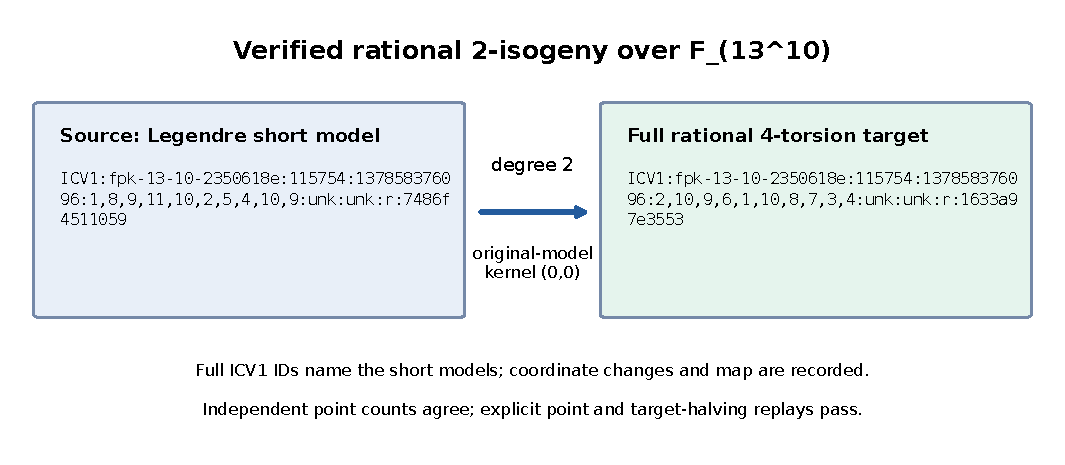
\includegraphics[width=\linewidth]{verified_isogeny.pdf}
\caption{A counted degree-10 example. Full source and target ICV1 IDs
name the short models; the retained records specify their coordinate
changes and the original-model map.}
\end{figure}

\section{Sources and validation}
The \href{https://pari.math.u-bordeaux.fr/dochtml/html/Elliptic_curves.html}{PARI reference}
documents \texttt{ellcard} on finite extensions and the available counting
algorithms. The existing \href{../THEOREM.tex}{norm-one theorem} supplies
the conductor obstruction at every size. The dated Markdown report links
all code, exact field and curve records, the cyclic audits, native tests,
failed preliminary attempts, and the persistent-service receipts.

\clearpage
\begin{landscape}
\begin{center}
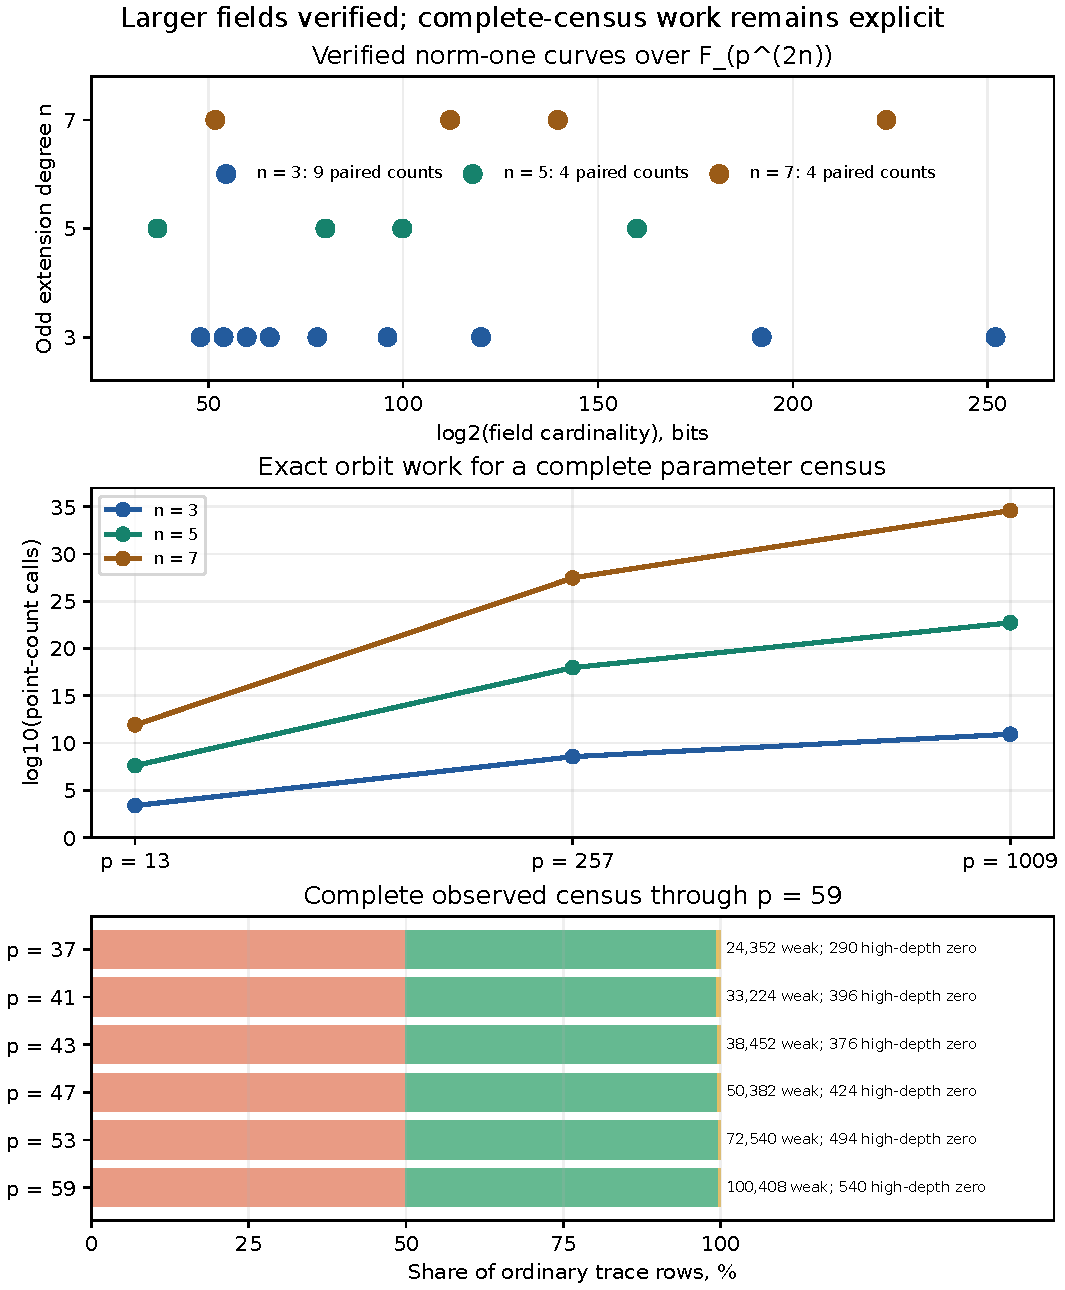
\includegraphics[width=\linewidth,height=0.88\textheight,keepaspectratio]{field_expansion.pdf}
\end{center}
\noindent Top: 17 completed point-count pairs; every plotted marker is a
measured field case. Bottom: exact orbit-call requirements from the
proved formula, displayed on a logarithmic scale. The graph does not
infer runtime or class reach from the positive controls.
\end{landscape}
\end{document}
